\clearpage
\newpage
%%%%%%%%%%%%%%%%%%%%%%%%%%%%%%%%%%%%%%%%%%%%%%%%%%%%%%%%%%%%%%%%%%
\section{E field using electrical diagram}\label{sec:elDiagram}
%%%%%%%%%%%%%%%%%%%%%%%%%%%%%%%%%%%%%%%%%%%%%%%%%%%%%%%%%%%%%%%%%%
The electric field strength in the LArIAT main drift volume can be determined knowing the voltage applied to the cathode, the voltage applied at the shield plane, and the distance between them. We assume the distance between the cathode and the shield plane to be 470 mm and any length contraction due to the liquid argon is negligibly small ($\sim 2$mm).

The voltage applied to the cathode can be calculated using Ohm's law and the circuit diagram shown in Figure \ref{fig:circuit}. The voltage supplied by the Glassman power supply during Run-I and Run-II was 23.5~kV. Between the Glassman power supply and the cathode was a set of two of filter pots for emergency power dissipation, one at each end of the feeder cable, each with an internal resistance of 40~M$\Omega$. 

Thus all that is needed to determine the electric field strength is the output current of the Glassman. However, an error in the values as recorded by Fermilab's Accelerator Controls Network (ACNET) was found during this investigation. As shown in Figure \ref{fig:currentMeasurement}, ACNET records an average current of 0.04172 mA from the power supply ($\sim$40$\mu$A).  This is now known to be unreliable, due to an uncalibrated scale factor. 

However, this number is inconsistent with the know resistance inside the TPC. The LArIAT TPC has four 1~G$\Omega$ resistors in parallel (250 M$\Omega$ equivalent) serving as the voltage divider across each of the 24 steps of the field cage. This means that the equivalent resistance across the whole TPC should be ~6~G$\Omega$. Thus the expected current out of the Glassman should be 
\begin{equation}
I_{expected} = \frac{V_{power supply}}{R_{Total}} = \frac{23.5 kV}{6.08 G\Omega} = 3.8 \mu A \approx 4 \mu A
\end{equation}

After further investigation it was concluded that the recording of the values in ACNET were likely mis-calibrated by a factor of 10 and thus the correct current to assume from the Glassman should be corrected to 0.00417 mA = 4$\mu$A.

\begin{figure}[hp]
\centering
\begin{minipage}{0.45\textwidth}
\centering
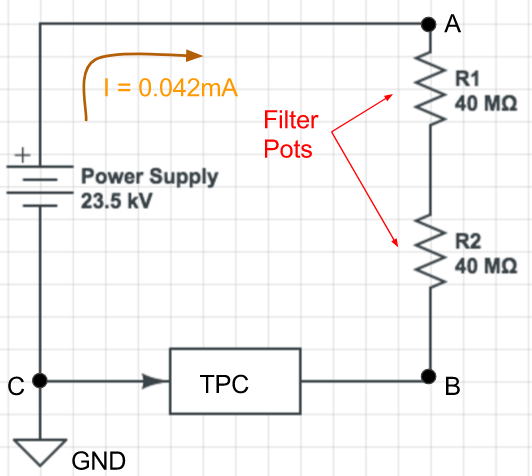
\includegraphics[width=3in]{images/CircuitLArIAT.png}
\caption{LArIAT HV simple schematics.}
\label{fig:circuit}
\end{minipage}\hfill
\begin{minipage}{0.45\textwidth}
\centering
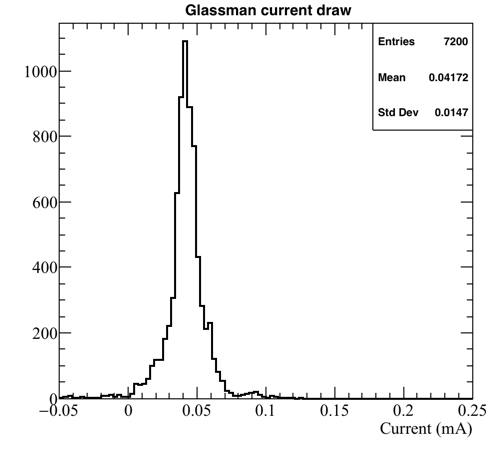
\includegraphics[width=3in]{images/glassman_current_20160525-30.png}
\caption{Current reading from the Glassman between May 25th and May 30th 2016 (typical Run2 conditions).}
\label{fig:currentMeasurement}
\end{minipage}
\end{figure}

Thus, using this corrected current, the voltage at the cathode is calculated as:

\begin{equation} V_{BC}=V_{PS} - I_{corrected}*R_{eq} = -23.5kV + 0.00417mA*80M\Omega = -23.17 kV, \label{eq:VBC}
\end{equation}
where I is the current and R$_{eq}$ is the equivalent resistor representing the two filter pots. The electric field, drift voltage and drift time are then calculated to be

\begin{equation}E_{filed} = \frac{V_{BC} - V_{shield}}{\Delta x} = 486.54 \textit{ V/cm}
\end{equation}
\begin{equation}v_{drift} = \mu E_{field} = 1.5097 \textit{ mm/$\mu$s}
\end{equation}
\begin{equation}t_{drift} = \frac{\Delta x}{v_{drift}} = 311.316 \textit{ $\mu$s.}
\end{equation}


